% !TEX program = xelatex

\documentclass{resume}
\usepackage{graphicx}
\usepackage{tabu}
\usepackage{multirow}
\usepackage{progressbar}
%\usepackage{zh_CN-Adobefonts_external} % Simplified Chinese Support using external fonts (./fonts/zh_CN-Adobe/)
%\usepackage{zh_CN-Adobefonts_internal} % Simplified Chinese Support using system fonts

\begin{document}
\pagenumbering{gobble} % suppress displaying page number

\Large{
  \begin{tabu}{ c l r }
   \multirow{5}{1in}{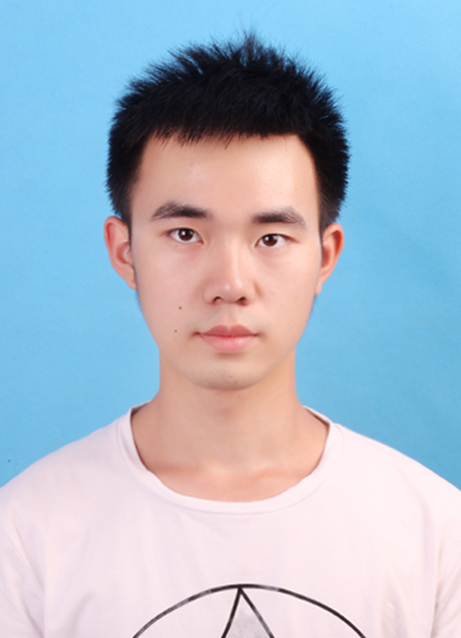
\includegraphics[width=0.88in]{avatar}} & \scshape{Feiyang Chen} & {Python~}\progressbar{0.90} \\
    & \email{feiyangchen98@gmail.com} & {Java~}\progressbar{0.90} \\
    & \phone{(+86) 178-0111-4068} & {C++~}\progressbar{0.80} \\
    &
    \github[Eurus-Holmes]{https://github.com/Eurus-Holmes}  & {Tensorflow~}\progressbar{0.7} \\
    & 
    \linkedin[Feiyang Chen]{https://www.linkedin.com/in/feiyangchen98} & {Pytorch~}\progressbar{0.7}
  \end{tabu}
}

\section{\faGraduationCap\ Education}
\datedsubsection{\textbf{Beijing Forestry University (BJFU)}, Beijing, China}{2016.9 -- 2020.6}
\textit{B.S. in Computer Science (CS), GPA: 89.34/100, Rank: 4/191 (top2\%)--->4/19}

\section{\faUsers\ Lab Experience}
\datedsubsection{\textbf{Iar, State Key Laboratory of CSAI, Tsinghua University}, Beijing, China}{2018.7 -- Present}
\role{Research Internship}{Research Topic: Multimodal Sentiment Analysis}
Submitted Paper: 
\begin{itemize}
	\item Journal of the Pattern Recognition Submitted
	\item AAAI2019: Reviews Scores: 775--->Meta-Reviews: rejected...
\end{itemize}

\datedsubsection{\textbf{Institute of Artificial Intelligence, Beijing Forestry University}, Beijing, China}{2018.4 -- Present}
\role{Program Leader}{2018 National College Student Innovation Training Program}
The project is expected to have the following achievements: 
\begin{itemize}
	\item Publish a paper by SCI or EI
	\item Text sentiment analysis website demo embedded in neural network model
\end{itemize}

\section{\faGithubAlt\ Projects Experience}
\datedsubsection{\textbf{WeChat applet: Play BJFU}}{2017.7 -- 2017.8}
\role{This is a WeChat small program that our "I Shangbeilin" team used for 30 days in the summer of the freshman year and completed self-study from zero. I'm the leader of the team.}

\begin{itemize}
	\item The total number of visits exceeded 10,000 times
	\item Admitted into the 6th National University SCT Innovation Works Conference
\end{itemize}

\datedsubsection{\textbf{LeetCode EveryDay (LCED)}}{2018.8 -- Present}
\url{https://github.com/Eurus-Holmes/LCED}

\role{Programmers are in a race with the Universe to create bigger and better idiot-proof programs, while the Universe is trying to create bigger and better idiots. 
	So, Join me! LeetCode EveryDay!}

% Reference Test
%\datedsubsection{\textbf{Paper Title\cite{zaharia2012resilient}}}{May. 2015}
%An xxx optimized for xxx\cite{verma2015large}
%\begin{itemize}
%  \item main contribution
%\end{itemize}

% \section{\faCogs\ Skills}
% \begin{itemize}[parsep=0.5ex]
%   \item Programming Languages: C == Python > C++ > Java
%   \item Platform: Linux
%   \item Development: Web, xxx
% \end{itemize}

% \section{\faHeartO\ Honors and Awards}
% \datedline{\textit{\nth{1} Prize}, Award on xxx }{Jun. 2013}
% \datedline{Other awards}{2015}

\section{\faInfo\ Miscellaneous}
\begin{itemize}[parsep=0.5ex]
	\item Blog: \url{http://blog.leanote.com/chenfeiyang}
	\item GitHub: \url{https://github.com/Eurus-Holmes}
	\item Leetcode: \url{https://leetcode.com/eurus-holmes/}

\end{itemize}

%% Reference
%\newpage
%\bibliographystyle{IEEETran}
%\bibliography{mycite}
\end{document}
